\section{Forschungsziele}


In der geplanten Wissenschaftlichen Arbeit, soll ein Konzept für ein sicheres Zahlungsverfahren 
für einen Click-and-Buy-Automat neben einem Campinplatz entwickelt werden. Solch ein Konzept kann
dazu beitragen, dass Campingplätze und die Gegend modernisiert werden und noch mehr Touristen 
angelockt werden. Bevor das Projekt jedoch umgesetzt werden kann, müssen noch wichtige Dinge 
beleuchtet werden. 


Der Zugang zum Netzwerk über das Glasfaser sollte immer gewährleistet werden, eine stabile Software, die 
den Qualitätsstandards entspricht, ein sicherer Umgang mit Kundendaten, der sich an spezifischen und
internationalen Richtlinien\footnote{Es gibt Regeln, die aussagen, was mit personenbezogenen Daten passieren
darf und was nicht \cite{refart:DSDS}.} orientiert, ein benutzerfreundliches System, das sich an verschiedenen 
Kundentypen, wie Alters- und Bildungsgruppe anpasst und letztlich ein kryptographisches Verfahren\footnote{Mit
Hilfe kryptographischer Verfahren, wie Verschlüsselung, sollen Daten vor unbefugtem Zugriff geschützt und sicher 
ausgetauscht werden \cite{refart:SLWK}.} für das bargeldlose Bezahlen, das die Vertraulichkeit sicherstellt.


\subsection{IT-Sicherheitsziel: Verfügbarkeit}
Um die Verfügbarkeit des Netzwerkzugangs für den Click-and-Buy-Automat zu gewährleisten, muss zum einen 
geprüft werden, ob die bereits vorhandenen Leitungen ausreichen, um dieses Projekt umsetzen zu können.
Die Vernetzung soll so aufgebaut sein, dass es auch in Regionen einwandfrei funktioniert, wo die
Infraestruktur nicht so ausgeprägt ist, wie in der Stadt. 


Die Software muss zudem so entwickelt werden, sodass diese eine geringe Ausfallquote aufweist, denn der
Automat soll rund um die Uhr betriebsbereit sein, um das Ziel der Verfügbarkeit des Systems nicht zu 
verletzen \cite{refbook:SWIS}.

\subsection{User-Experience}
Zudem soll das System so entwickelt werden, sodass auch Digital Non-Natives\footnote{Bezeichnet
eine Person, die in der Kindheit ohne Informationstechnologien und ohne dem Internet aufgewachsen ist 
und eine Welt mit digitalen Medien nicht kennt \cite{misc:MSND}.}, die Möglichkeit \cite{refart:QWDN} haben
das System einfach bedienen zu können. Die Kunden sollten also nicht von Informationen überladen werden, 
sondern es sollte einfache Ein- und Ausgaben geben. Eine Umfrage aus dem Jahr 2019 \cite{periodical:AdCJ}
zeigt, dass sich besonderes ältere Menschen \cite{periodical:AdCJ} für solch eine Urlaubsmöglichkeit entscheiden.
Das spielt für den Erfolg des Konzeptes eine entscheidene Rolle, dass auch sie mit dem Automat umgehen können. 
Deshalb sollten die Bedürfnisse und Einschränkungen dieser Altergruppe besonders berücksichtigt werden, um ihr 
Vertrauen zu gewinnen \cite{refart:HLAU} und hauptsächlich gegen Social-Engineering\footnote{Beim Social-Engineering 
nutzt der Täter den ``Faktor Mensch'' als vermeintlich schwächstes Glied der Sicherheitskette aus, um seine kriminelle
Absicht zu verwirklichen.\cite{booklet:BSSE}} Angriffe zu schützen. Die Auswahl der Tests trägt dazu bei, dass die 
Zufriedenheit und die Akzeptanz gewährleistet wird, sodass jeder potenziellen Endnutzer das System bedienen kann 
\cite{refbook:IASE}.


\vfill
\begin{figure}[H]
    \centering{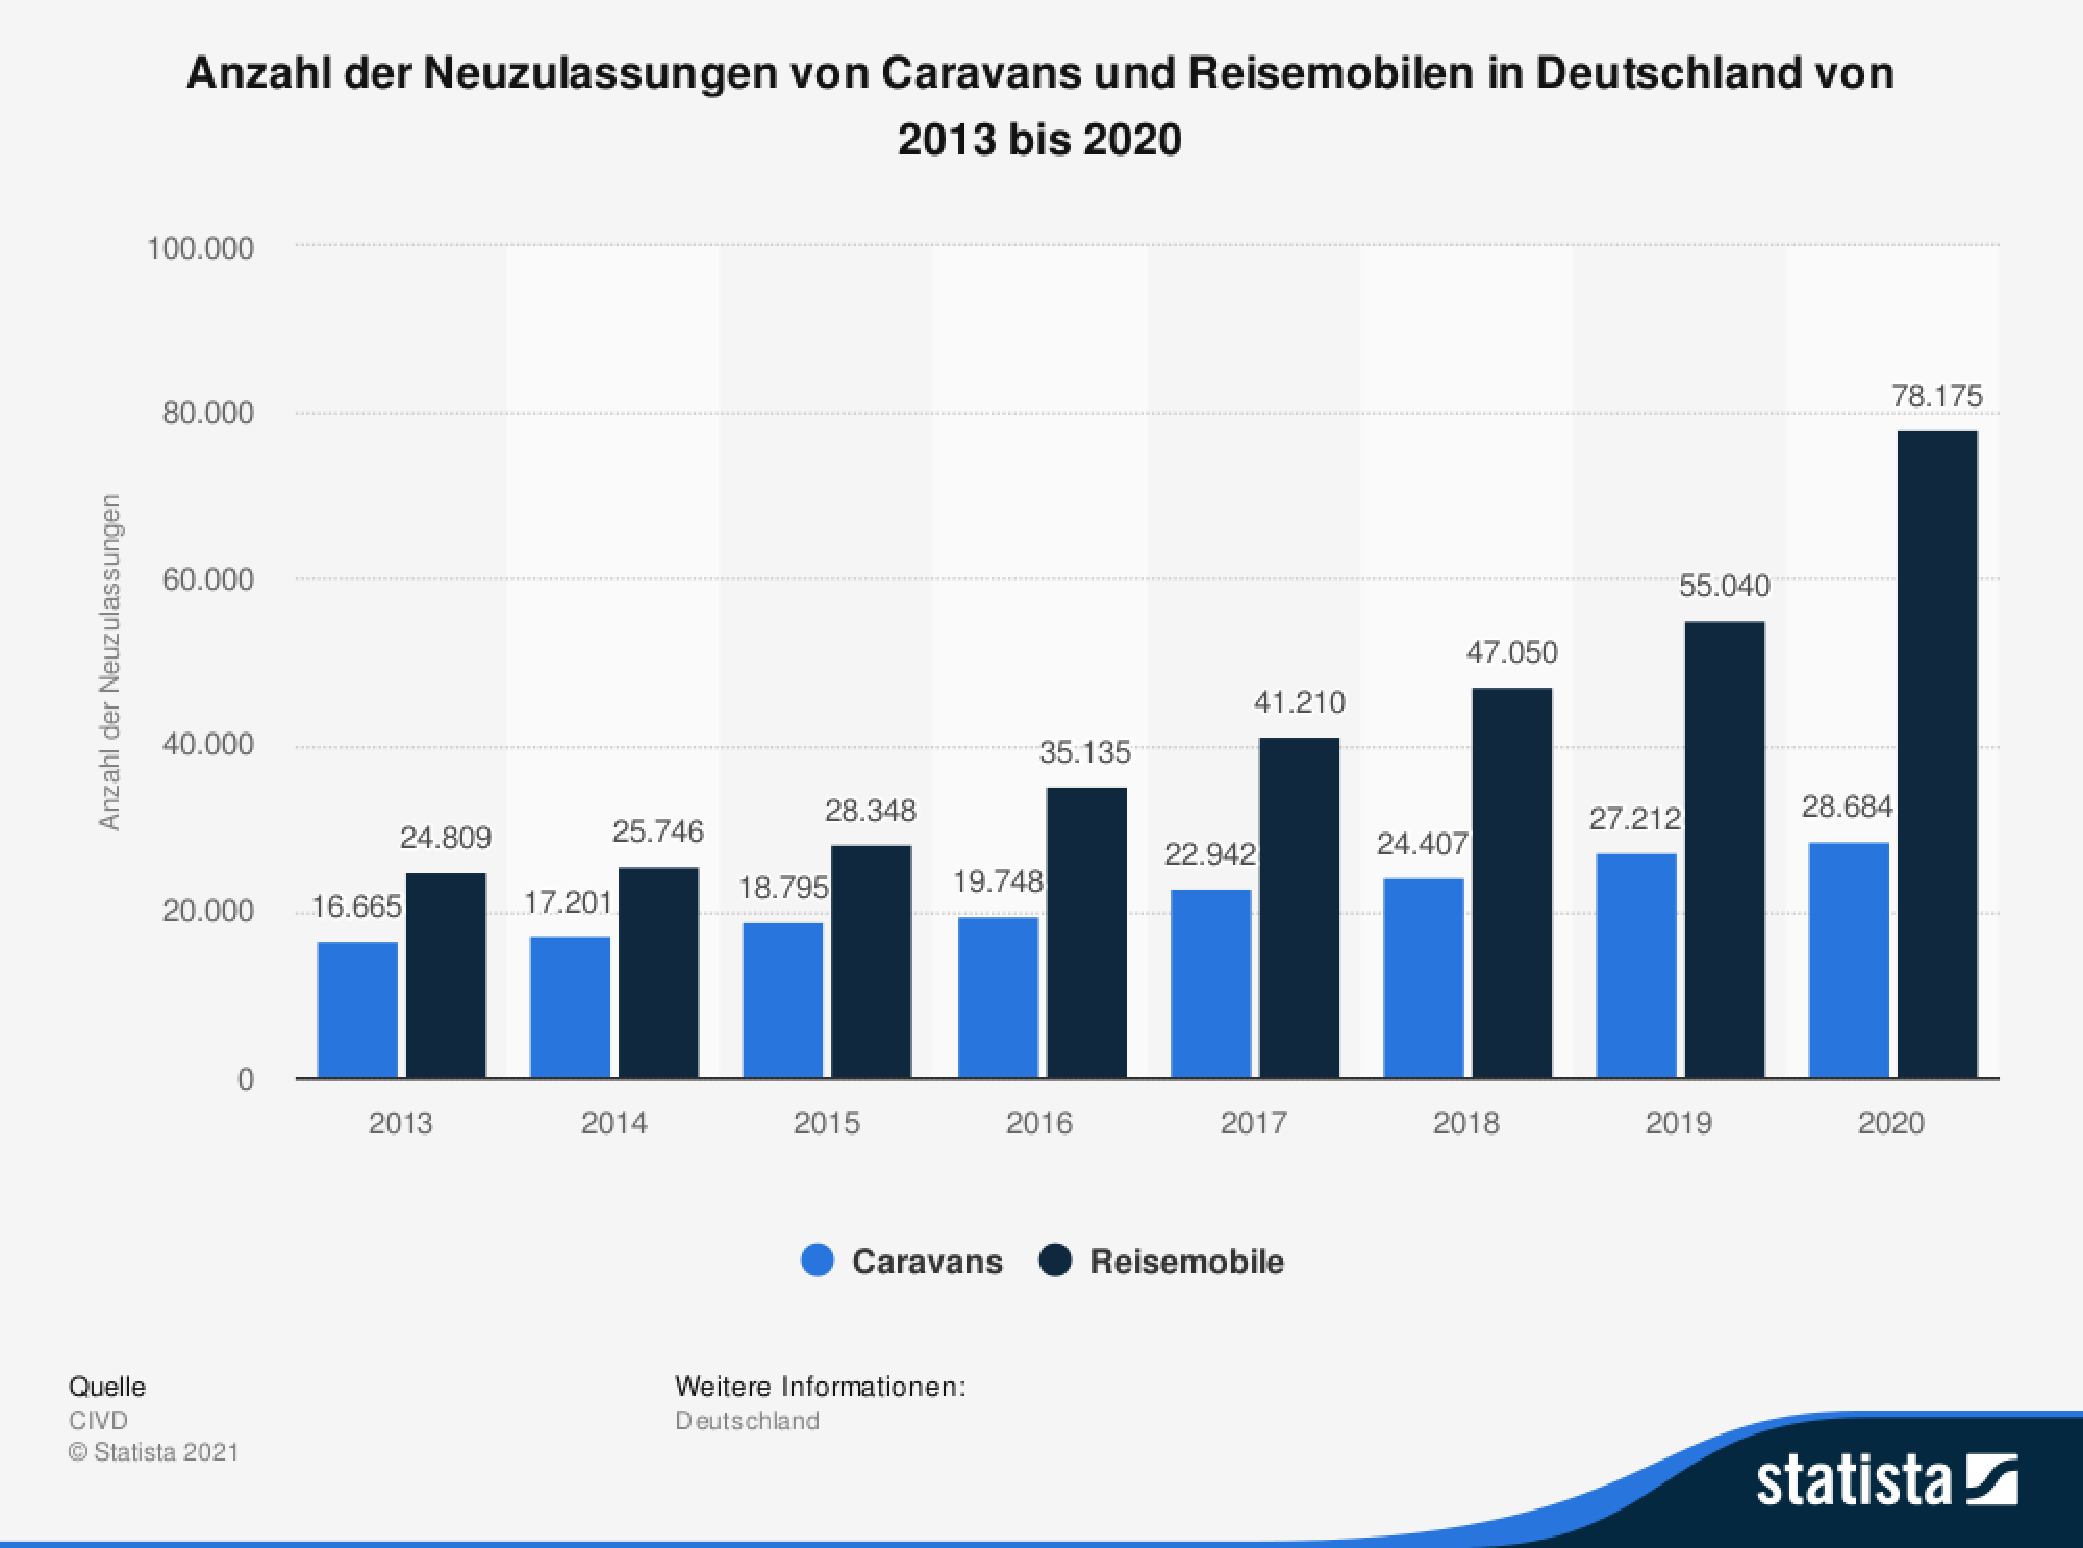
\includegraphics[width=12cm]{Bilder/periodical_ANST}}
    \caption{Altergruppe von Campinurlauberm im Jahr 2019 \\ Quelle: Graefe, 2019}
    \label{fig:periodical_AdCJ}
\end{figure}
% \cite{periodical:AdCJ}


Außerdem spielt die Sicherheit bei den bargeldlosen Zahlungsvorgängen eine große Rolle und sollte deshalb 
höchste Priorität haben. Verschiedene aktuelle Beispiele von Cyberangriffe zeigen, dass der Umgang mit
solchen Daten, kritisch zu sehen ist \cite{booklet:BKCB}. 

\subsection{IT-Sicherheitsziel: Vertraulichkeit}
Es wird oft von Situationen in den Medien berichtet, bei denen Kunden ihr Geld verloren haben oder dessen
personenbezogenen Daten missbraucht wurden. In seltenen Fällen sogar von der eigenen Regierung, weil das System 
nicht ausreichend gegen Angriffe geschützt wurde. In dieser Hinsicht sollten bei der Entwicklung spezifische 
und klare Richtlinien berücksichtig werden, sodass der sichere Umgang mit personenbezogenen Daten gewährleistet ist 
\cite{refart:TRVR}. Um diese Vertraulichkeitsverletzung zu vermeiden, spielt die Konziperiung von sicheren 
bargeldlosen Zahlungsmethoden eine wesentliche Rolle in diesem Artikel. 